\chapter{Oracle APEX HR-2}

\section{Mengurutkan Repositori Interaktif}
\begin{enumerate}
    \item{Klik Spreadsheet}
\begin{figure}[!htbp]
    \centering
    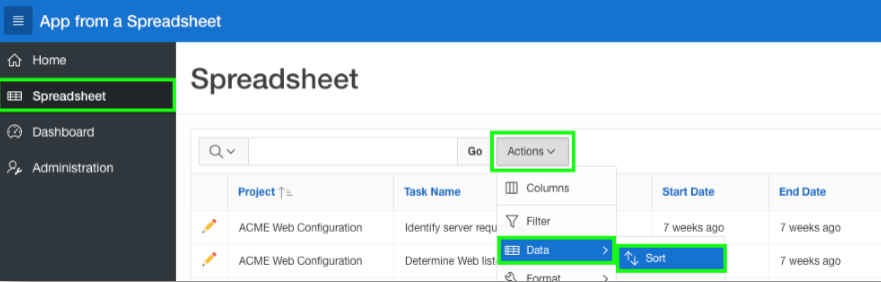
\includegraphics[scale=0.5]{section/gambar_bab2/spreadsheet.png}
    \label{penanda}
\end{figure}
    \item{Klik actions, lalu pilih data dan sort. Untuk 1 pilihlah start date, yang kedua pilih end date, dan klik apply.}
\end{enumerate} 

\section{Cara Menambahkan Perhitungan}
\begin{enumerate}
    \item{Klik actions, lalu pilih data, dan pilih compute}
    \item{Selanjutnya label kolom masuk budget v cost dan pilih format mask 5,243.10}
    \item{Pada kolom Computation Expression, ketik I-H dan klik apply seperti gambar berikut ini.}
\begin{figure}[!htbp]
    \centering
    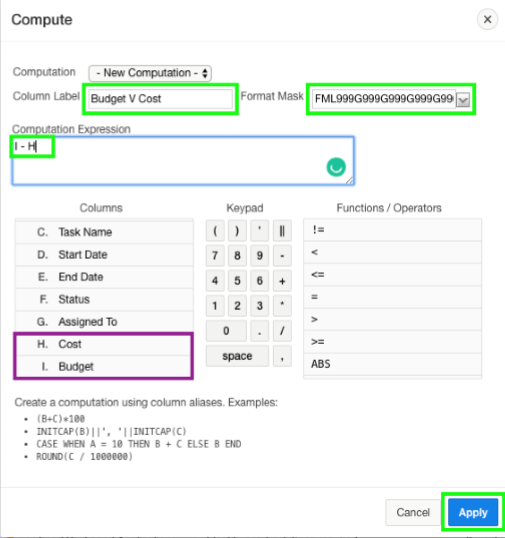
\includegraphics[scale=0.5]{section/gambar_bab2/budget.png}
    \label{penanda}
\end{figure}
\end{enumerate}

\section{Cara Menambahkan Chart}
\begin{enumerate}
    \item{Pada menu actions, pilih chart}
    \item{Pada atribut label pilih project, value pilih **budget v cost, function pilih sum, sort pilih label - ascending, dan orientation pilih horizontal.}
    \item{Setelah selesai memilih semua, klik apply.}
\begin{figure}[!htbp]
    \centering
    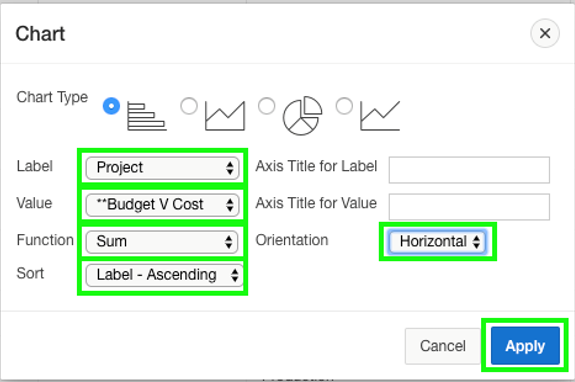
\includegraphics[scale=0.5]{section/gambar_bab2/chart.png}
    \label{penanda}
\end{figure}
\end{enumerate}

\section{Cara Menyimpan Laporan}
\begin{enumerate}
    \item{Seperti biasa pada menu actions, pilih report dan save report.}
    \item{Untuk menyimpan laporan, pilih report, dan save report.}
\begin{figure}[!htbp]
    \centering
    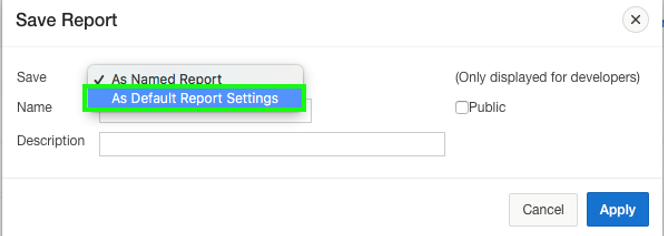
\includegraphics[scale=0.5]{section/gambar_bab2/SR.png}
    \label{penanda}
\end{figure}
    \item{Pilih alternative pada default type dan data review pada name.}
    \item{Terakhir, klik apply.}
\begin{figure}[!htbp]
    \centering
    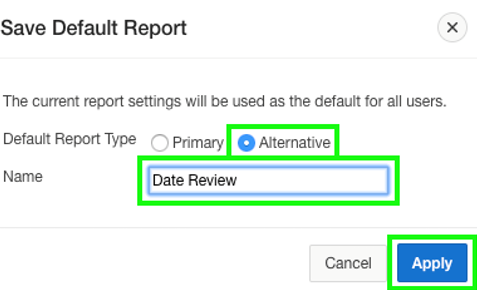
\includegraphics[scale=0.5]{section/gambar_bab2/SDR.png}
    \label{penanda}
\end{figure}
\end{enumerate}

\section{Restrict atau Membatasi Status}
\begin{enumerate}
    \item{Pada runtime environment, klik edit icon di record, lalu halaman modal akan ditampilkan.}
    \item{Klik Quick Edit pada Developer Toolbar dan klik kiri pada item status.}
    \item{Halaman designer akan menampilkan status item.}
\begin{figure}[!htbp]
    \centering
    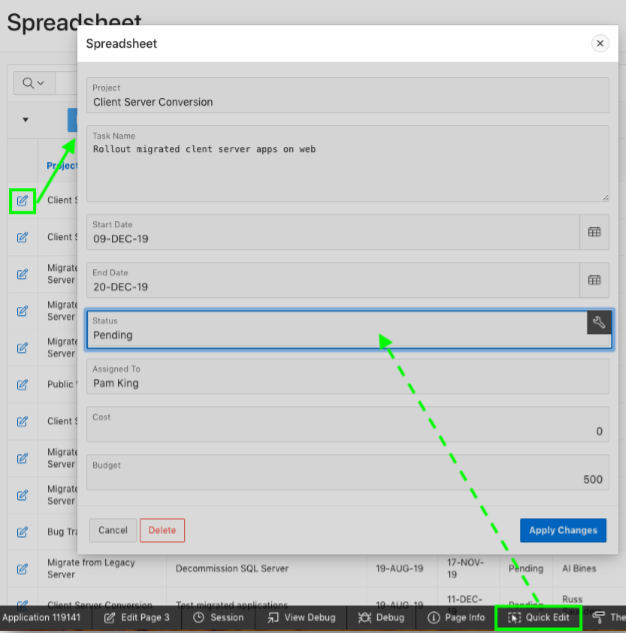
\includegraphics[scale=0.5]{section/gambar_bab2/status.png}
    \label{penanda}
\end{figure}
    \item{Pilih tipe select list pada halaman designer di dalam property editor dan klik kanan.}
    \item{Lalu memilih tipe SQL query pada list of values dan klik code editor.}
\begin{figure}[!htbp]
    \centering
    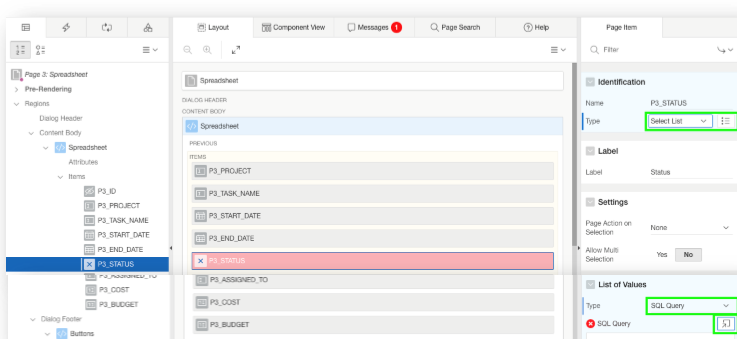
\includegraphics[scale=0.5]{section/gambar_bab2/status2.png}
    \label{penanda}
\end{figure}
    \item{Ketik tulisan berikut ini di code editor:}
    \item{Lalu klik validate dan oke jika selesai.}
\begin{figure}[!htbp]
    \centering
    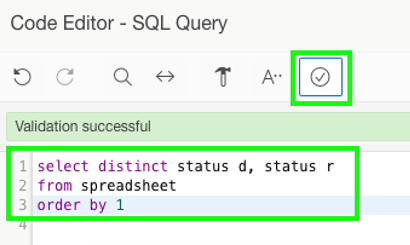
\includegraphics[scale=0.5]{section/gambar_bab2/status3.png}
    \label{penanda}
\end{figure} 
    \item{Pilih no pada display extra values dan ketik -Select Status- pada null value display.}
    \item{Setelah itu klik simpan.}
    
\begin{figure}[!htbp]
    \centering
    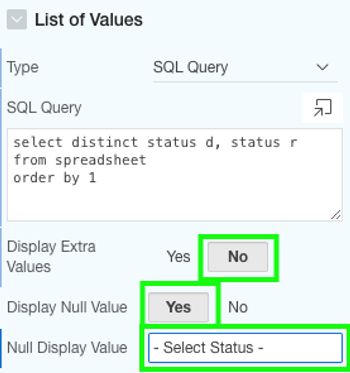
\includegraphics[scale=0.5]{section/gambar_bab2/status4.png}
    \label{penanda}
\end{figure}
\end{enumerate}

\section{Menjalankan Aplikasi}
\begin{enumerate}
    \item{Untuk menjalankan aplikasi,arahkan lagi ke runtime environment, lalu refresh browser yang digunakan, dan edit record. Klik status dan ubah menjadi closed}
    
\begin{figure}[!htbp]
    \centering
    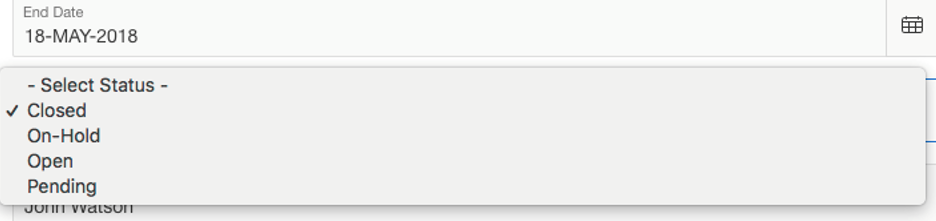
\includegraphics[scale=0.5]{section/gambar_bab2/status5.png}
    \label{penanda}
\end{figure}
\end{enumerate}

\section{Menambahkan Kalender}
\begin{enumerate}
    \item{Untuk menambahkan kalender, balik lagi ke runtime environment}
    \item{Pada halaman app builder, arahkan ke halaman utama, dan klik create page untuk membuat halaman.}
    
\begin{figure}[!htbp]
    \centering
    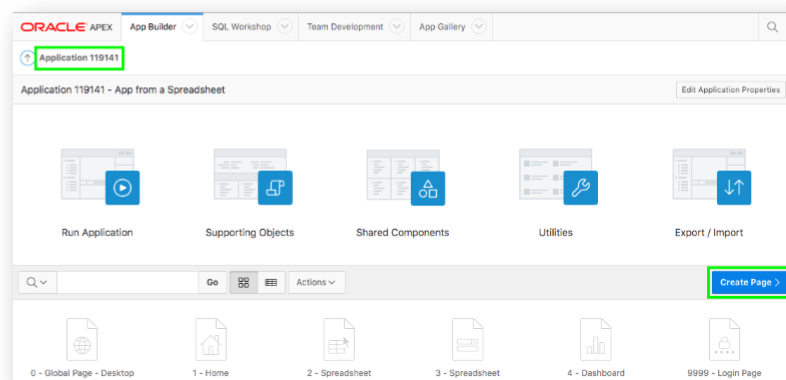
\includegraphics[scale=0.5]{section/gambar_bab2/kalender.png}
    \label{penanda}
\end{figure}
    \item{Pilih kalender dan isi atribut halaman.}
    
\begin{figure}[!htbp]
    \centering
    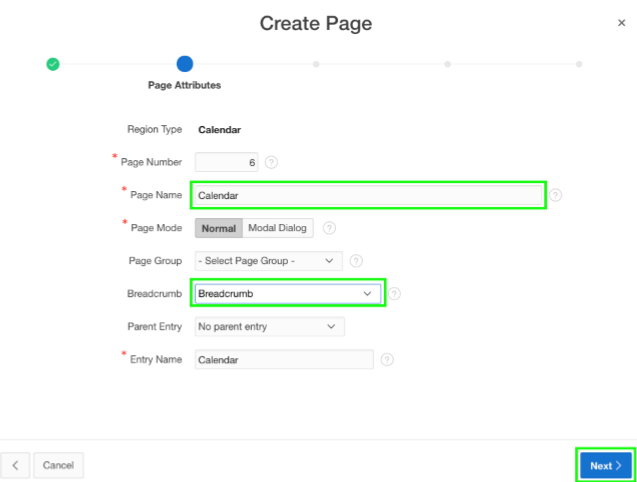
\includegraphics[scale=0.5]{section/gambar_bab2/kalender3.png}
    \label{penanda}
\end{figure}

    \item{Selanjutnya pilih create a new navigation menu entry dan klik next.}
    \item{Pada menu source pilih SPREADSHEET (table) dan klik next.}
    \item{Lalu klik create setelah mengatur display column dan end date column.}
    
\begin{figure}[!htbp]
    \centering
    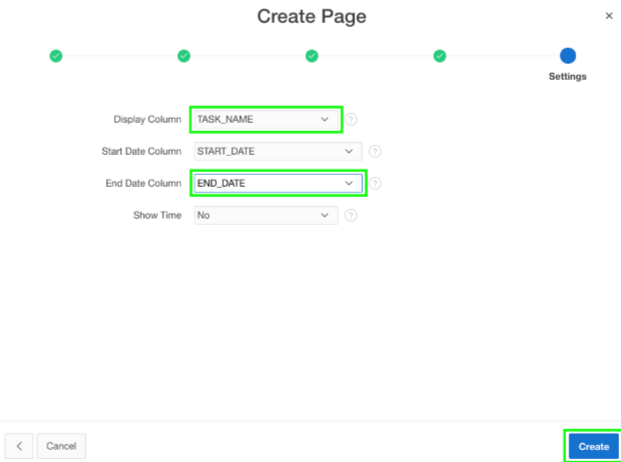
\includegraphics[scale=0.5]{section/gambar_bab2/kalender6.png}
    \label{penanda}
\end{figure}
\end{enumerate}

\section{Mengupdate Form dengan Link Kalender}
\begin{enumerate}
    \item{Klik attributes dibawah calender pada halaman designer. Selanjutnya klik view/edit link.}
    \item{Pada atribute pilih 3}
    \item {Pada set items, ubah name dan value}
    \item {Atur Clear Cache menjadi 3, dan klik OK.}
    
\begin{figure}[!htbp]
    \centering
    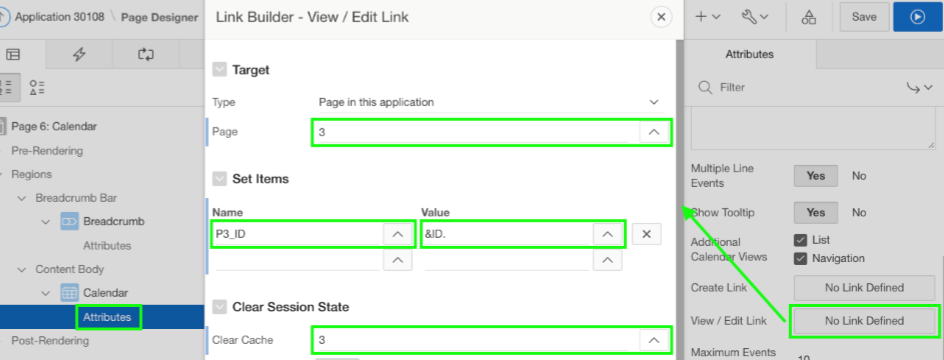
\includegraphics[scale=0.5]{section/gambar_bab2/kalender7.png}
    \label{penanda}
\end{figure}

    \item {Lalu, klik save and run. Kalender sudah berjalan.}
    
\begin{figure}[!htbp]
    \centering
    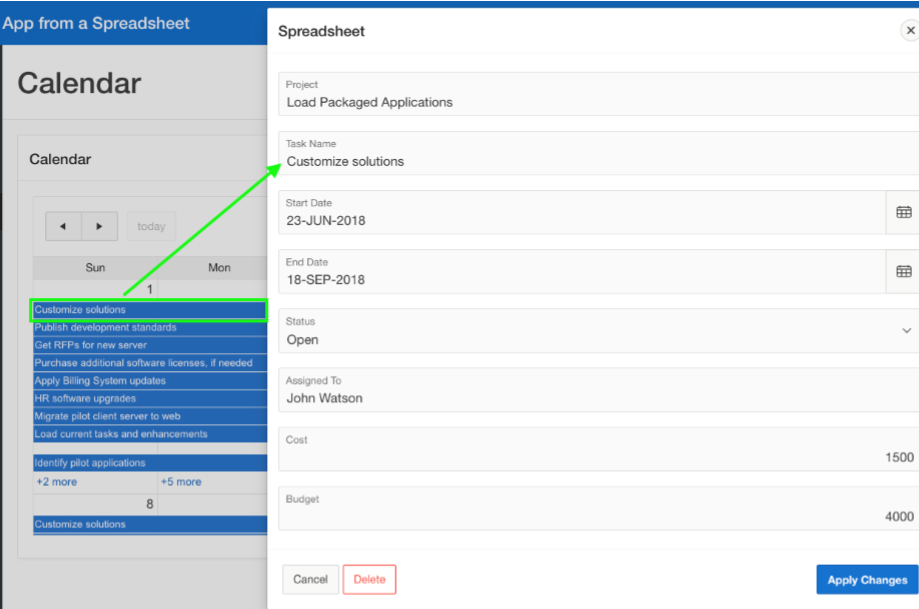
\includegraphics[scale=0.5]{section/gambar_bab2/kalender8.png}
    \label{penanda}
\end{figure}
\end{enumerate}